% !TeX root = ../main.tex

\section{Pictures}

\subsection{Simplest centered}
\begin{figure}[!ht]
    \begin{minipage}{\linewidth}
        \centering
        \makebox[\textwidth][c]{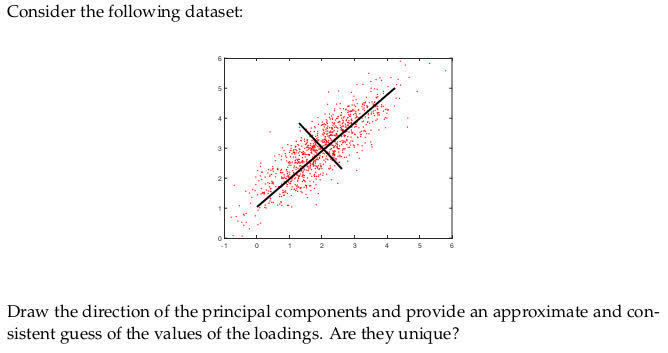
\includegraphics[width=1\textwidth]{images/Bias-Variance Tradeoff_01.png}}%
        %\caption{Nielsen's heuristics evaluation summary}
        %\label{BarsNielsenCrop}
    \end{minipage}
\end{figure}

\subsection{Adjacent centered}
\begin{center}
    
\includegraphics[width=0.3\textwidth]{images/Bias-Variance Tradeoff_03.png}
    \hspace{1em}
    
\includegraphics[width=0.3\textwidth]{images/Bias-Variance Tradeoff_04.png}
\end{center}

\subsection{Captioned figure}
I'm referring to figure \ref{refer_sample}
\begin{figure}[!ht]
    \begin{minipage}[c]{\linewidth}
        \centering
        \makebox[\textwidth][c]{
\includegraphics[width=0.6\textwidth]{images/Bias-Variance Tradeoff_02.png}}%
        \captionsetup{justification=centering}
        \caption{This is a caption}
        \label{refer_sample}
    \end{minipage}
\end{figure}

\subsection{One caption per multiple images}
I'm referring to figure \ref{refer_sample_2}
\begin{figure}[!ht]
    \centering
    \subfloat[][\centering Case 1]{{
\includegraphics[width=7cm]{images/Bias-Variance Tradeoff_03.png} }}%
    \qquad
    \subfloat[][\centering Case 2]{{
\includegraphics[width=7cm]{images/Bias-Variance Tradeoff_04.png} }}%
    \captionsetup{justification=centering}
    \caption{VC dimension < 5}%
    \label{refer_sample_2}%
\end{figure}